%!TEX root = <main.tex>
\vspace{-1mm}
\section{Setup and Preliminaries}\label{sec:preliminaries}
We now state our problem formally and explain our assumptions.
We then formalize the dataflow of the layers of a CNN, since these are required for understanding our techniques in Sections 3 and 4.
Table~\ref{table:preliminaries_symbols} lists our notation.
\eat{
Finally we briefly explain the Structural Similarity Index (SSIM) which is used to quantify the quality of the generated sensitivity heat maps.
}

\vspace{-2mm}
\subsection{Problem Statement and Assumptions}\label{sec:problem}

We are given a CNN $f$ that has a sequence (or DAG) of \textit{layers} $l$, each of which has a \textit{tensor transformation function} $T_{:l}$. We are also given the image $\mathcal{I}_{:img}$ for which the occlusion-based explanation (OBE) is desired, the class label $L$ predicted by $f$ on $\mathcal{I}_{:img}$, an occlusion patch $\mathcal{P}$ in RGB format, and occlusion patch \textit{stride} $S_{\mathcal{P}}$. We are also given a set of patch positions $G$ constructed either automatically or manually with a visual interface interactively. The OBE workload is as follows: produce a 2-D heat map $M$, wherein each value corresponds to a position in $G$ and has the prediction probability of $L$ by $f$ on the occluded image $\mathcal{I}^{'}_{x,y:img}$ (i.e., superimpose occlusion patch on image) or zero otherwise.
More precisely, we can describe the OBE workload with the following logical statements:

\vspace{-7mm}
\begin{align}
\label{eqn:mheight}
W_M =&~ \lfloor(\texttt{width}(\mathcal{I}_{:img}) - \texttt{width}(\mathcal{P}) + 1)/S_\mathcal{P}\rfloor\\
\label{eqn:mwidth}
H_M =&~ \lfloor(\texttt{height}(\mathcal{I}_{:img}) - \texttt{height}(\mathcal{P}) + 1)/S_\mathcal{P}\rfloor\\
M \in&~ \mathcal{\rm I\!R}^{H_M \times W_M}\\
\forall~ (x,y) \in&~ G:\\
\label{eqn:patchimpose}
& \mathcal{I}^{'}_{x,y:img} \leftarrow \mathcal{I}_{:img} ~ \bm\circ_{(x,y)} ~ \mathcal{P} \\
\label{eqn:outputval}
& M[x,y] \leftarrow f(\mathcal{I}^{'}_{x,y:img})[L]
\vspace{-5mm}
\end{align}

Steps~(\ref{eqn:mheight}) and~(\ref{eqn:mwidth}) calculate the dimensions of the heat map $M$.
Step~(\ref{eqn:patchimpose}) superimposes $\mathcal{P}$ on $\mathcal{I}_{:img}$ with its top left corner placed on the $(x,y)$ location of $\mathcal{I}_{:img}$.
Step~(\ref{eqn:outputval}) calculates the output value at the $(x,y)$ location by performing CNN inference for $\mathcal{I}^{'}_{x,y:img}$ using $f$ and picks the prediction probability of $L$.
Steps~(\ref{eqn:patchimpose}) and~(\ref{eqn:outputval}) are performed \textit{independently} for every occlusion patch position in $G$.
In the \textit{non-interactive} mode, $G$ is initialized to $G = [0, H_M) \times [0, W_M)$. Intuitively, this represents the set of all possible occlusion patch positions on $\mathcal{I}_{:img}$, which yields a full heat map. In the \textit{interactive} mode, the user may manually place the occlusion patch only at a few locations at a time, yielding partial heat maps.

\begin{table}[t]
  \centering
  \scalebox{0.8}{\begin{tabular}{p{2cm}p{7.5cm}}
    \toprule
    \textbf{Symbol} & \textbf{Meaning}\\
    \midrule \midrule
    $f$ & Given deep CNN; input is an image tensor; output is a probability distribution over class labels\\
    \midrule
    $L$ & Class label predicted by $f$ for the original image $\mathcal{I}_{:img}$\\
    \midrule
    $T_{:l}$ & Tensor transformation function of layer $l$ of the given CNN $f$\\
    \midrule
    $\mathcal{P}$ & Occlusion patch in RGB format\\
    \midrule
    $S_\mathcal{P}$ & Occlusion patch striding amount\\
    \midrule
    $G$ & Set of occlusion patch superimposition positions on $\mathcal{I}_{:img}$ in (x,y) format\\
    \midrule
    $M$ & Heat map produced by the OBE workload\\
    \midrule
    $H_M,W_M$ & Height and width of $M$\\
    \midrule
    $\bm\circ_{(x,y)}$ & Superimposition operator. $A~\circ_{(x,y)}~B$, superimposes $B$ on top of $A$ starting at $(x,y)$ position\\
    \midrule
    $\mathcal{I}_{:l} ~(\mathcal{I}_{:img})$ & Input tensor of layer $l$ (Input Image)\\
    \midrule
    $\mathcal{O}_{:l}$ & Output tensor of layer $l$\\
    \midrule
    $C_{\mathcal{I}:l},H_{\mathcal{I}:l},W_{\mathcal{I}:l}$ & Depth, height, and width of input of layer $l$\\
    \midrule
    $C_{\mathcal{O}:l},H_{\mathcal{O}:l},W_{\mathcal{O}:l}$ & Depth, height, and width of output of layer $l$\\
    \midrule
    $\mathcal{K}_{conv:l}$ & Convolution filter kernels of layer $l$\\
    \midrule
    $\mathcal{B}_{conv:l}$ & Convolution bias value vector of layer $l$\\
    \midrule
    $\mathcal{K}_{pool:l}$ & Pooling filter kernel of layer $l$\\
    \midrule
    $H_{\mathcal{K}:l},W_{\mathcal{K}:l}$ & Height and width of filter kernel of layer $l$\\
    \midrule
    $S_{:l}; S_{x:l}; S_{y:l}$ & Filter kernel striding amounts of layer $l$; $S_{:l} \equiv (S_{x:l}, S_{y:l})$, strides along width and height dimensions\\
    \midrule
    $P_{:l}; P_{x:l}; P_{y:l}$ & Padding amounts of layer $l$; $P_{:l} \equiv (P_{x:l}, P_{y:l})$, padding along width and height dimensions\\
    % $Q (Q_{inc})$ & Total FLOPS count with full (incremental) inference\\
    % \midrule
    % $L$ & Set of convolution layers in a CNN\\
    % \midrule
    \bottomrule
  \end{tabular}}
    \caption{Notation used in this paper.}
\label{table:preliminaries_symbols}
\vspace{-8mm}
\end{table}

\eat{%TODO: This part should go up to the introduction
The focus of this work is on the occlusion based deep CNN explainability approach \cite{zeiler2014visualizing}, which is widely used by practitioners in several domains including healthcare, sociology, security, and agriculture \cite{kermany2018identifying, islam2017abnormality, mohanty2016using, arbabzadah2016identifying, wang2017deep}.
}
We assume the CNN is used for classification (or regression), since only such applications typically use OBE. One could create CNNs that predict an image ``segmentation'' instead, but labeling image segments for training such CNNs is tedious and expensive. Thus, most recent applications of CNNs in healthcare, sociology, and other domains rely on classification CNNs and use OBE~\cite{kermany2018identifying, islam2017abnormality, mohanty2016using, arbabzadah2016identifying, wang2017deep}. Other approaches to explain CNN predictions have been studied, but since they are orthogonal to our focus, we summarize them in the appendix due to space constraints.
We assume $f$ is from a roster of well-known deep CNNs; we currently support VGG16, ResNet18, and InceptionV3. We think this is a reasonable start, since most recent OBE applications use only such well-known CNNs from model zoos~\cite{caffemodelzoo, tfmodelzoo}. But we note that our techniques are generic enough to apply to any CNN; we leave support for arbitrary CNNs to future work.

\begin{figure*}[t]
\vspace{-2mm}
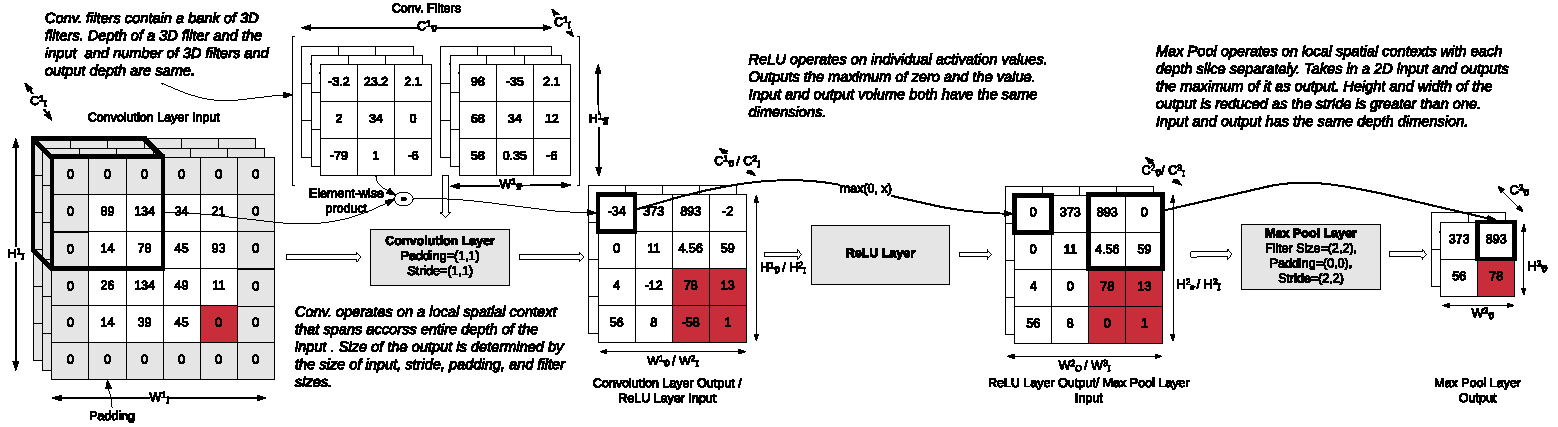
\includegraphics[width=\textwidth]{images/cnn_simplified}
\vspace{-6mm}
\caption{Simplified illustration of the key layers of a typical CNN. The highlighted cells (dark/red background) show how a small local spatial context in the first input propagates through subsequent layers. (a) Convolution layer (for simplicity sake, bias addition is not shown). (b) ReLU Non-linearity layer. (c) Pooling layer (max pooling). Notation is explained in Table~\ref{table:preliminaries_symbols}.}
\vspace{-2mm}
\label{fig:cnn_simplified}
\end{figure*}

\subsection{Dataflow of CNN Layers}\label{sec:cnn_internals}
CNNs are organized as \textit{layers} of various types, each of which transforms a tensor (multidimensional array, typically 3-D) into another tensor: \textit{Convolution} uses image filters from graphics to extract features, but with parametric filter weights (learned during training); \textit{Pooling} subsamples features in a spatial-aware manner; \textit{Batch-Normalization} normalizes the output tensor; \textit{Non-Linearity} applies an element-wise non-linear function (e.g., ReLU); \textit{Fully-Connected} is an ordered collection of perceptrons~\cite{dlbook}. The output tensor of a layer can have a different width, height, and/or depth than the input. An image can be viewed as a tensor, e.g., a 224$\times$224 RGB image is a 3-D tensor with width and height 224 and depth 3. A Fully-Connected layer converts a 1-D tensor (or a ``flattened'' 3-D tensor) to another 1-D tensor. For simplicity of exposition, we group CNN layers into 3 main categories based on the \textit{spatial locality} of how they transform a tensor: (1) Transformations with a \textit{global context}, e.g., Fully-Connected; (2) Transformations at the granularity of \textit{individual elements}, e.g., ReLU or Batch Normalization; and (3) Transformations at the granularity of a \textit{local spatial context}, e.g. Convolution or Pooling.

\vspace{2mm}
\noindent \textbf{Global context granularity.} 
Such layers convert the input tensor holistically into an output tensor without any spatial context, typically with a full matrix-vector multiplication.
Fully-Connected is the only layer of this type. Since every element of the output will likely be affected by the entire input, such layers do not offer a major opportunity for faster incremental computations. Thankfully, Fully-Connected layers typically arise only as the last layer(s) in deep CNNs (and never in some recent deep CNNs), and they typically account for a negligible fraction of the total computational cost. Thus, we do not focus on such layers for our optimizations.
%The computational cost of a Full-Connected transformation is proportional to the product of the size of the input and output 1-D tensors.

\vspace{2mm}
\noindent \textbf{Individual element granularity.} 
Such layers apply a ``map()'' function on the elements of the input tensor, as Figure~\ref{fig:cnn_simplified}(b) illustrates.
Thus, the output has the same dimensions as the input. Non-Linearity (e.g., with ReLU) falls under this category. The computational cost is proportional to the ``volume'' of the input tensor (product of the dimensions). If the input is incrementally updated, only the corresponding region of the output will be affected. Thus, incremental inference for such layers is straightforward. The computational cost of the incremental computation is proportional to the volume of the updated region.

\vspace{2mm}
\noindent \textbf{Local spatial context granularity.}
Such layers perform weighted aggregations of slices of the input tensor, called \textit{local spatial contexts}, by multiplying them with a \textit{filter kernel} (a tensor of weights). Thus, input and output tensors can differ in width, height, and depth. If the input is incrementally updated, the region of the output that will be affected is not straightforward to ascertain--this requires non-trivial and careful calculations due to the overlapping nature of how filters get applied to local spatial contexts. Both Convolution and Pooling fall under this category. Since such layers typically account for the bulk of the computational cost of deep CNN inference, enabling incremental inference for such layers in the OBE context is a key focus of this paper (Section 3). The rest of this section explains the machinery of the dataflow in such layers using our notation. Section 3 then uses this machinery to explain our optimizations.
% Convolution layers are the most important type of layer in the CNN architecture which also contributes to most of the computational cost.

\vspace{2mm}
\noindent \textbf{Dataflow of Convolution Layers.}
A layer $l$ has $C_{\mathcal{O}:l}$ 3-D filter kernels arranged as a 4-D array $\mathcal{K}_{conv:l}$, with each having a smaller spatial width $W_{\mathcal{K}:l}$ and height $H_{\mathcal{K}:l}$ than the width $W_{\mathcal{I}:l}$ and height $H_{\mathcal{I}:l}$ of the input tensor $\mathcal{I}_{:l}$ but the same depth $C_{\mathcal{I}:l}$. During inference, $c^{th}$ filter kernel is ``strided'' along the width and height dimensions of the input to produce a 2-D ``activation map'' $A_{:c}=(a_{y,x:c})\in \mathcal{\rm I\!R}^{H_{\mathcal{O}:l} \times~ W_{\mathcal{O}:l}}$ by computing element-wise products between the kernel and the local spatial context and adding a bias value as per Equation (\ref{eqn:elementwise_product}). The computational cost of each of these small matrix products is proportional to the volume of the filter kernel. All the 2-D activation maps are then stacked along the depth dimension to produce the output tensor $\mathcal{O}_{:l} \in \mathcal{\rm I\!R}^{C_{\mathcal{O}:l} \times H_{\mathcal{O}:l} \times W_{\mathcal{O}:l}}$.
% as per Equation (\ref{eqn:conv_operator}). 
Figure~\ref{fig:cnn_simplified} (a) presents a simplified illustration of this layer.

\vspace{-4mm}
\begin{align}
\label{eqn:elementwise_product}
\begin{split}
a_{y,x:c} =& \sum_{k=0}^{C_{\mathcal{I}:l} } \sum_{j=0}^{H_{\mathcal{K}:l}-1} \sum_{i=0}^{W_{\mathcal{K}:l}-1} \mathcal{K}_{conv:l}[c, k, j, i] \\
& \quad \times \mathcal{I}_{:l}[k,y-\floor{\frac{H_{\mathcal{K}:l} }{2}}+j,x-\floor{\frac{W_{\mathcal{K}:l} }{2}}+i] \\
& \quad + \mathcal{B}_{conv:l}[c]
\end{split}
\vspace{-8mm}
\end{align}

\eat{
\begin{align}
\label{eqn:conv_operator}
\begin{split}
\mathcal{O}_{:l} = [A_{:0}, A_{:1}, ... , A_{(C_{\mathcal{O}:l}-1)}]
\end{split}
\end{align}
}

% \eat{
% \begin{align}
% \begin{split}
% \text{Input Volume}:&~ \mathcal{I} \in \mathcal{\rm I\!R}^{C_{\mathcal{I}} \times H_{\mathcal{I}} \times W_{\mathcal{I}}}\\
% \text{Convolution Filters}:&~ \mathcal{K}_{conv} \in \mathcal{\rm I\!R}^{C_{\mathcal{O}} \times C_{\mathcal{I}} \times H_{\mathcal{K}} \times W_{\mathcal{K}}}\\
% \text{Convolution Bias Vector}:&~ \mathcal{B}_{conv} \in \mathcal{\rm I\!R}^{C_{\mathcal{O}}}\\
% \text{Output Volume}:&~ \mathcal{O} \in \mathcal{\rm I\!R}^{C_{\mathcal{O}} \times H_{\mathcal{O}} \times W_{\mathcal{O}}}
% \end{split}
% \end{align}

% \begin{equation}
% \label{eqn:conv_operator}
% \begin{split}
% \mathcal{O}[c,y,x] &= \sum_{k=0}^{C_{\mathcal{I}}} \sum_{j=0}^{H_\mathcal{K}-1} \sum_{i=0}^{W_\mathcal{K}-1} \mathcal{K}_{conv}[c, k, j, i] \\ & \quad \quad \quad \times \mathcal{I}[k,y-\floor{\frac{H_\mathcal{K}}{2}}+j,x-\floor{\frac{W_\mathcal{K}}{2}}+i] + \mathcal{B}[c]
% \end{split}
% \end{equation}
% }

\vspace{2mm}
\noindent \textbf{Dataflow of Pooling Layers.} 
Such layers behave essentially like Convolution layers but with a fixed (not learned) 2-D filter kernel $\mathcal{K}_{pool:l}$. These kernels aggregate a local spatial context to compute its maximum or average element. But unlike Convolution, Pooling operates independently on the depth slices of the input tensor.
% The two main variations of pooling layers are max pooling (takes the maximum value from the local spatial context) and average (takes the average value from the local spatial context) pooling.
It takes as input a 3-D tensor $\mathcal{O}_{l}$ of depth $C_{\mathcal{I}:l}$, width $W_{\mathcal{I}:l}$, and height $H_{\mathcal{I}:l}$. It produces as output a 3-D tensor $\mathcal{O}_{:l}$ with the same depth $C_{\mathcal{O}:l}=C_{\mathcal{I}:l}$ but a different width of $W_{\mathcal{O}:l}$ and height $H_{\mathcal{O}:l}$. The filter kernel is typically strided over more than one pixel at a time. Thus, $W_{\mathcal{O}:l}$ and $H_{\mathcal{O}:l}$ are usually smaller than $W_{\mathcal{I}:l}$ and $H_{\mathcal{I}:l}$, respectively. Figure~\ref{fig:cnn_simplified}(c) presents a simplified illustration of this layer.
Overall, both Convolution and Pooling layers have a similar dataflow along the width and height dimensions, while differing on the depth dimension. Since OBE only concerns the width and height dimensions of the image and subsequent tensors, we can treat both these types of layers in a unified manner for our optimizations.

% Similar to Convolution, Pooling operation can be formally defined as follows:

% \begin{align}
% \text{Pool Filters}:&~ \mathcal{K}_{pool} \in \mathcal{\rm I\!R}^{H_{\mathcal{K}} \times W_{\mathcal{K}}}
% \end{align}

% \begin{equation}
% \label{eqn:pool_operator}
% \begin{split}
% \mathcal{O}[c,y,x] &= \sum_{j=0}^{H_\mathcal{K}-1} \sum_{i=0}^{W_\mathcal{K}-1} \mathcal{K}_{pool}[j, i] \\ & \quad \quad \quad \times \mathcal{I}[c,y-\floor{\frac{H_\mathcal{K}}{2}}+j,x-\floor{\frac{W_\mathcal{K}}{2}}+i]
% \end{split}
% \end{equation}

\vspace{2mm}
\noindent \textbf{Relationship between Input and Output Dimensions.}
For Convolution and Pooling layers, $W_{\mathcal{O}:l}$ and $H_{\mathcal{O}:l}$ are determined solely by $W_{\mathcal{I}:l}$ and $H_{\mathcal{I}:l}$, $W_{\mathcal{K}:l}$ and $H_{\mathcal{K}:l}$, and two other parameters that are specific to that layer: \textit{stride} $S_{:l}$ and \textit{padding} $P_{:l}$. Stride is the number of pixels by which the filter kernel is moved at a time; it can differ along the width and height dimensions: $S_{x:l}$ and $S_{y:l}$, respectively. But in practice, most CNNs have $S_{x:l} = S_{y:l}$. Typically, $S_{x:l} \leq W_{\mathcal{K}:l}$ and $S_{y:l} \leq H_{\mathcal{K}:l}$. In Figure~\ref{fig:cnn_simplified}, the Convolution layer has $S_{x:l} = S_{y:l} = 1$, while the Pooling layer has $S_{x:l} = S_{y:l} = 2$. For some layers, to help control the dimensions of the output to be the same as the input, one ``pads'' the input with zeros along the width and height dimensions. \textit{Padding} $P_{:l}$ captures how much such padding extends these dimensions; once again, the padding values can differ along the width and height dimensions: $P_{x:l}$ and $P_{y:l}$. In Figure~\ref{fig:cnn_simplified} (a), the Convolution layer has $P_{x:l} = P_{y:l} = 1$. Given all these parameters, the width (similarly height) of the output tensor is given by the following formula:

\vspace{-4mm}
\begin{align}
\begin{split}
W_{\mathcal{O}:l} = (W_{\mathcal{I}:l} - W_{\mathcal{K}:l} + 1 + 2\times P_{x:l})/S_{x:l} \\
% ^lH_{\mathcal{O}} = (^lH_{\mathcal{I}} - ^lH_\mathcal{K} + 1 + 2\times ^lP_y)/^lS_y
\end{split}
\end{align}

\vspace{2mm}
\noindent \textbf{Computational Cost of Inference.}
Deep CNN inference is computationally expensive. Convolution layers typically account for a bulk of the cost ($90\%$ or more)~\cite{cavigelli2017cbinfer}. Thus, we can roughly estimate the computational cost of inference by counting the number of \textit{fused multiply-add} (FMA) floating point operations (FLOPs) needed for the Convolution layers.
% and ignore the computational cost of other layers (e.g. Pooling, Fully-Connected).
For example, applying a Convolution filter with dimensions $(C_{\mathcal{I}:l} , H_{\mathcal{K}:l} , W_{\mathcal{K}:l})$ to compute one element of the output tensor requires $C_{\mathcal{I}:l} \cdot H_{\mathcal{K}:l} \cdot  W_{\mathcal{K}:l}$ FLOPs, with each FLOP corresponding to one FMA. Thus, the total computational cost $Q_{:l}$ of a layer that produces output $\mathcal{O}_{:l}$ of dimensions $(C_{\mathcal{O}:l} , H_{\mathcal{O}:l} , W_{\mathcal{O}:l})$ and the total computational cost $Q$ of the entire set of Convolution layers of a given CNN $f$ can be calculated as per Equations~(\ref{eqn:full_local}) and~(\ref{eqn:full_all}).

\vspace{-4mm}
\begin{align}
\label{eqn:full_local}
Q_{:l} =&~ (C_{\mathcal{I}:l} \cdot H_{\mathcal{K}:l} \cdot W_{\mathcal{K}:l})  (C_{\mathcal{O}:l} \cdot H_{\mathcal{O}:l} \cdot W_{\mathcal{O}:l})\\
\label{eqn:full_all}
Q =&~ \sum_{l~\mathit{in}~f}Q_{:l}
\end{align}


\eat{
\subsection{Estimating the Quality of Generated Approximate Heat Maps}

When applying approximate inference optimizations \system~ sacrifices the the accuracy/quality of the generated heat map in favor of faster execution.
To measure this drop of accuracy we use Structural Similarity (SSIM) Index~\cite{wang2004image} which is one of the widely used approaches to measure the \textit{human perceived difference} between two similar images.
When applying SSIM index we treat the original heat map as the reference image with no distortions and the perceived image similarity of the \system~generated heat map is calculated with reference to it.
The generated SSIM index is a value between $-1$ and $1$, where $1$ corresponds to perfect similarity.
% It is important to note that, even though SSIM index value of 1 corresponds to perfect similarity, other values doesn't necessarily imply same level of perceived quality across different image pairs.
% However, if the original images are closely similar, such as in chest X-ray images, it can be assumed that this condition will hold.
Typically SSIM index values in the range of $0.90-0.95$ are used in practical applications such as image compression and video encoding as at the human perception level they produce indistinguishable distortions.
For more details on SSIM Index method, we refer the reader to the original SSIM Index paper~\cite{wang2004image}.
}

